\documentclass[compress, 12pt]{beamer}

\let\Tiny=\tiny % fuck you beamer !

\usepackage[utf8]{inputenc}
\usepackage[T1]{fontenc}
\usepackage[french]{babel}
\usepackage{graphicx}
\usepackage{soul}
\usepackage{palatino}

\usetheme{Luebeck}

\useoutertheme{infolines}

\setbeamertemplate{navigation symbols}{}
\title{IA41 - Force 3}
\subtitle{Soutenance de projet}
\author[]{Tao Sauvage \and Julien Voisin \and Robin Faury}
\institute[UTBM]{Université de Technologie de Belfort Montbéliard}
\logo{
\includegraphics[width=.05\textwidth]{./pix/sym_plateau}}

\newcommand{\link}[2] {
\item[#1] \scriptsize #2 \normalsize
}

\AtBeginSection{
  \begin{frame}{Plan}<beamer>
    \tableofcontents[currentsection,currentsubsection]
  \end{frame}
  \addtocounter{framenumber}{-1}
}

\begin{document}

\begin{frame}
	\titlepage
\end{frame}


\begin{frame}{Plan}
    \tableofcontents
\end{frame}


\section{Analyse}

\begin{frame}{Un jeu de société}
  \begin{figure}
    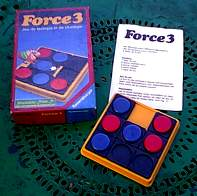
\includegraphics[height=0.6\textheight]{./pix/plateau}
    \centering
    \caption{Boîte de teeko}
  \end{figure}
\end{frame}


\begin{frame}{Modélisation de la partie}
  \begin{figure}
    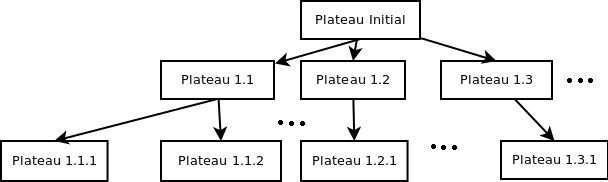
\includegraphics[width=\textwidth]{./pix/arbre}
    \centering
    \caption{Un arbre représentant une partie}
  \end{figure}
\end{frame}


\begin{frame}{Évaluation d'un plateau}
    \begin{columns}
        \begin{column}{.2\textwidth}
            
\includegraphics[width=\textwidth]{./pix/sym_plateau}
        \end{column}
        \begin{column}{.6\textwidth}
            \begin{block}{Fonction d'évaluation}
                $$-100 \leq evaluation(plateau) \leq 100$$
            \end{block}
            \begin{block}{Pondération en fonction du nombre de pions alignés:}
                \begin{description}
                    \item[1 pion seul:] 1 point 
                    \item[2 pions alignés:] 5 point
                    \item[3 pions alignés:] 100 points
                \end{description}
            \end{block}
        \end{column}
    \end{columns}
\end{frame}

\begin{frame}{Évaluation d'un plateau : Exemple}
    \begin{columns}
        \begin{column}[l]{0.5\textwidth}
            \begin{figure}
                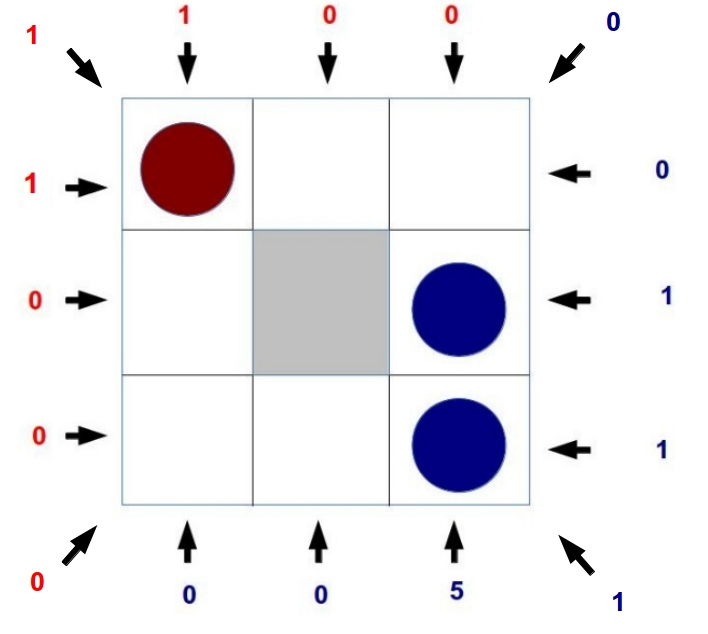
\includegraphics[width=1.05\textwidth, height=4.5cm]{./pix/evaluation}
                \centering
                \caption{Evaluation d'un plateau}
            \end{figure}
        \end{column}
        
        \begin{column}[r]{0.5\textwidth}
            \begin{description}
                \item[Rouge:] $1 + 1 + 1 = 3$
                \item[Bleu:] $5 + 1 + 1 + 1 = 8$
                \item[Évaluation Bleu:] $8 -3 = 5$
            \end{description}
        \end{column}

  \end{columns}
\end{frame}

\begin{frame}{Méthode de résolution}
  \begin{figure}
    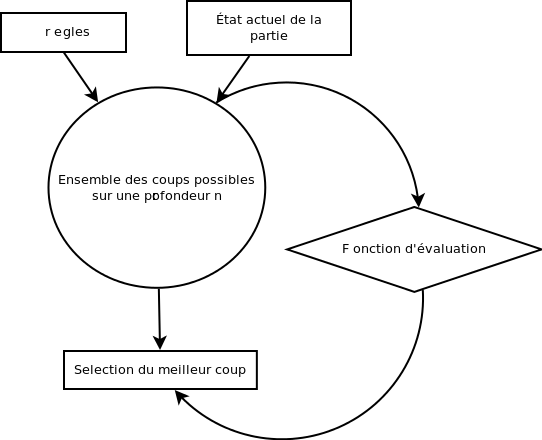
\includegraphics[height=0.7\textheight]{./pix/methode}
    \centering
    \caption{Méthode de résolution}
  \end{figure}
\end{frame}


\begin{frame}{Algorithme utilisé}
  \begin{figure}
    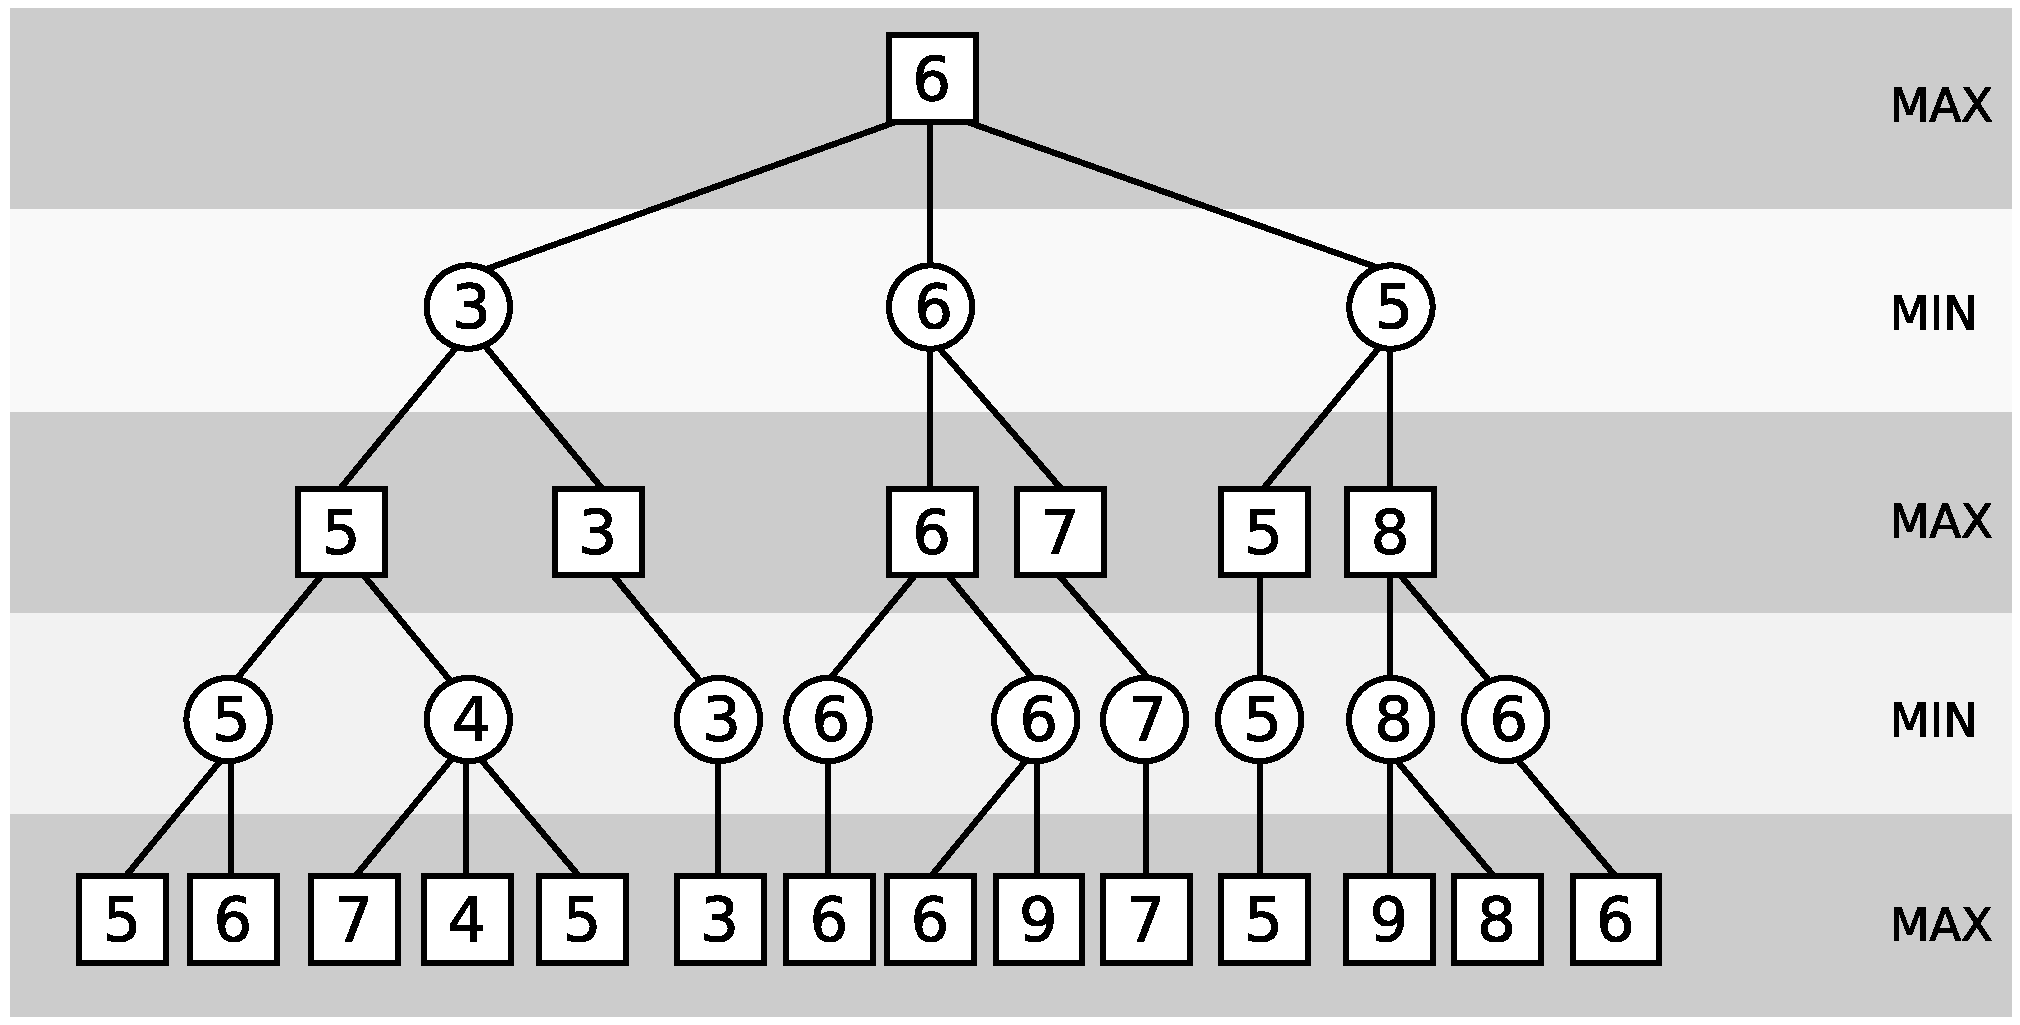
\includegraphics[width=\textwidth]{pix/minimax}
    \centering
    \caption{MiniMax}
  \end{figure}
\end{frame}

\begin{frame}{Algorithme utilisé}
  \begin{figure}
    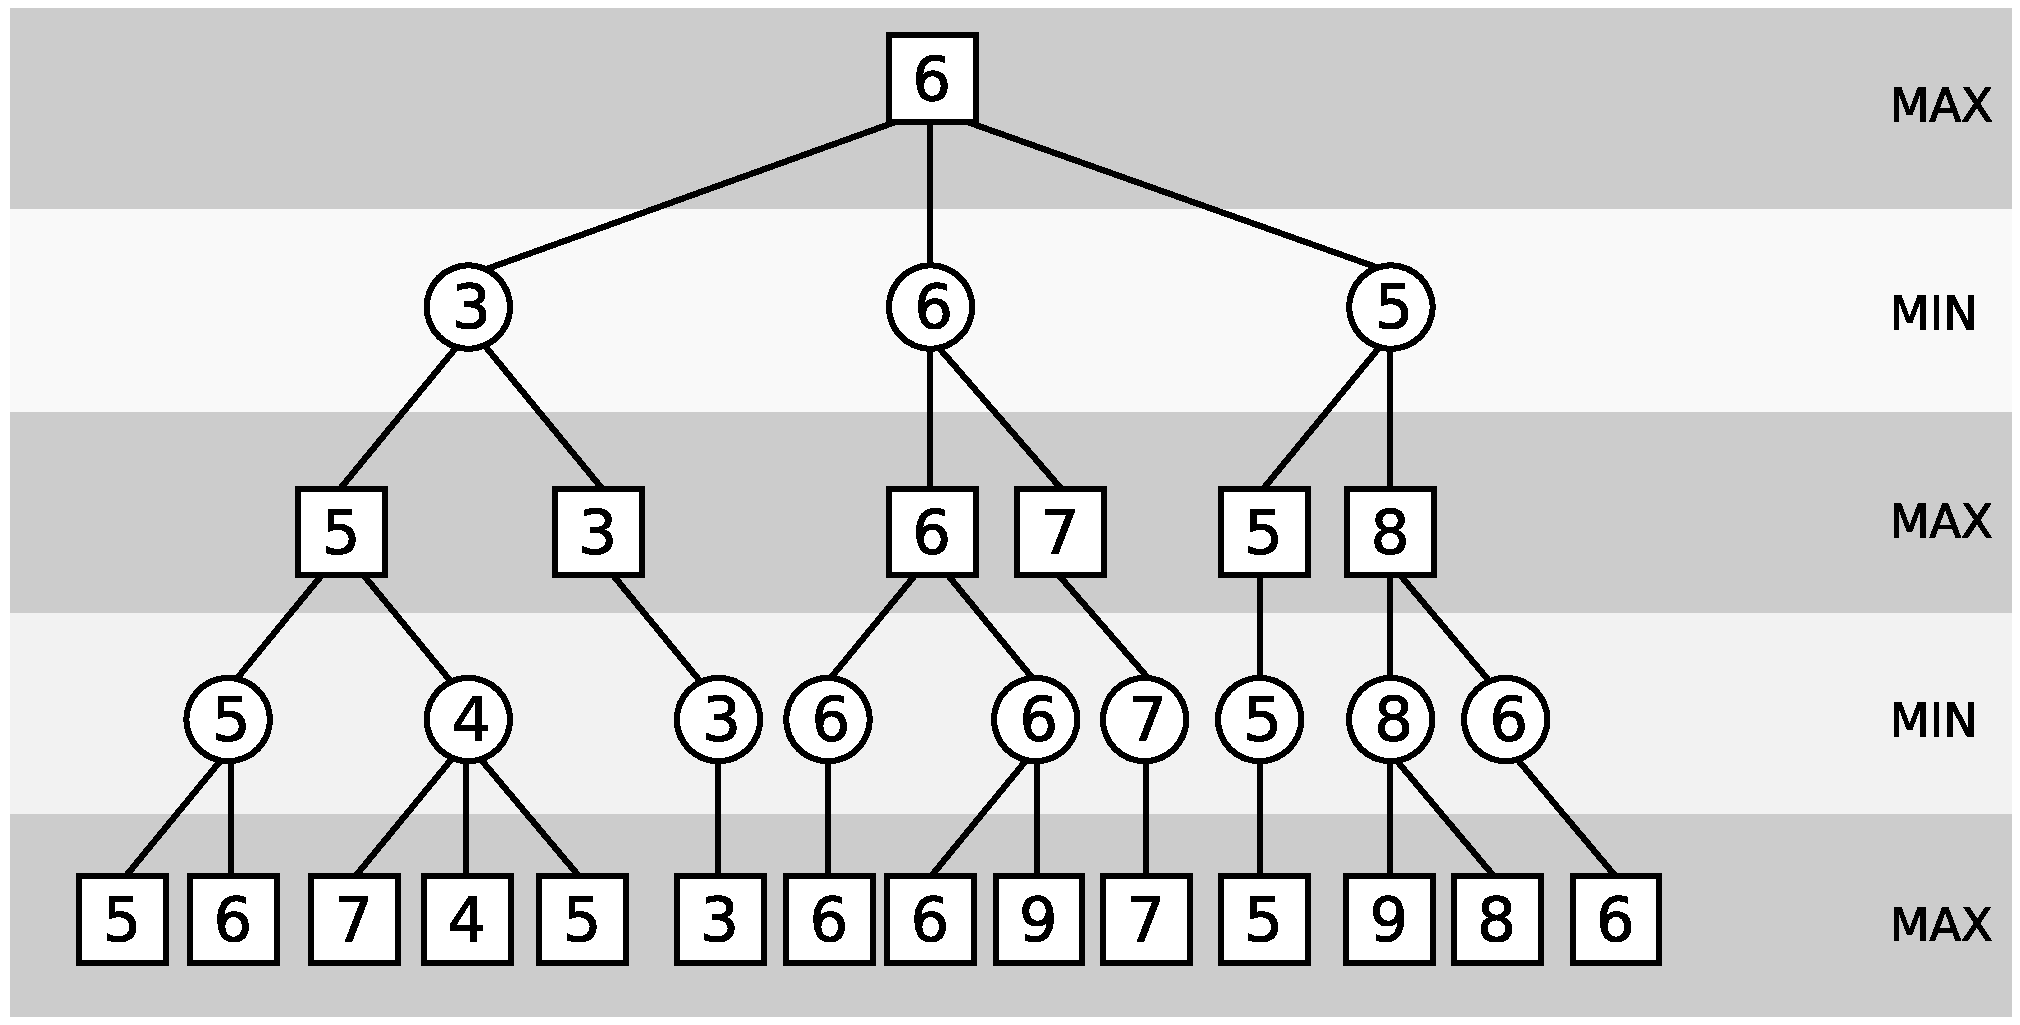
\includegraphics[width=\textwidth]{pix/minimax}
    \centering
    \caption{\st{Minimax} Négamax}
  \end{figure}
  \begin{center}
  MIN = - MAX
  \end{center}
\end{frame}

\begin{frame}{Algorithme utilisé}
  \begin{figure}
    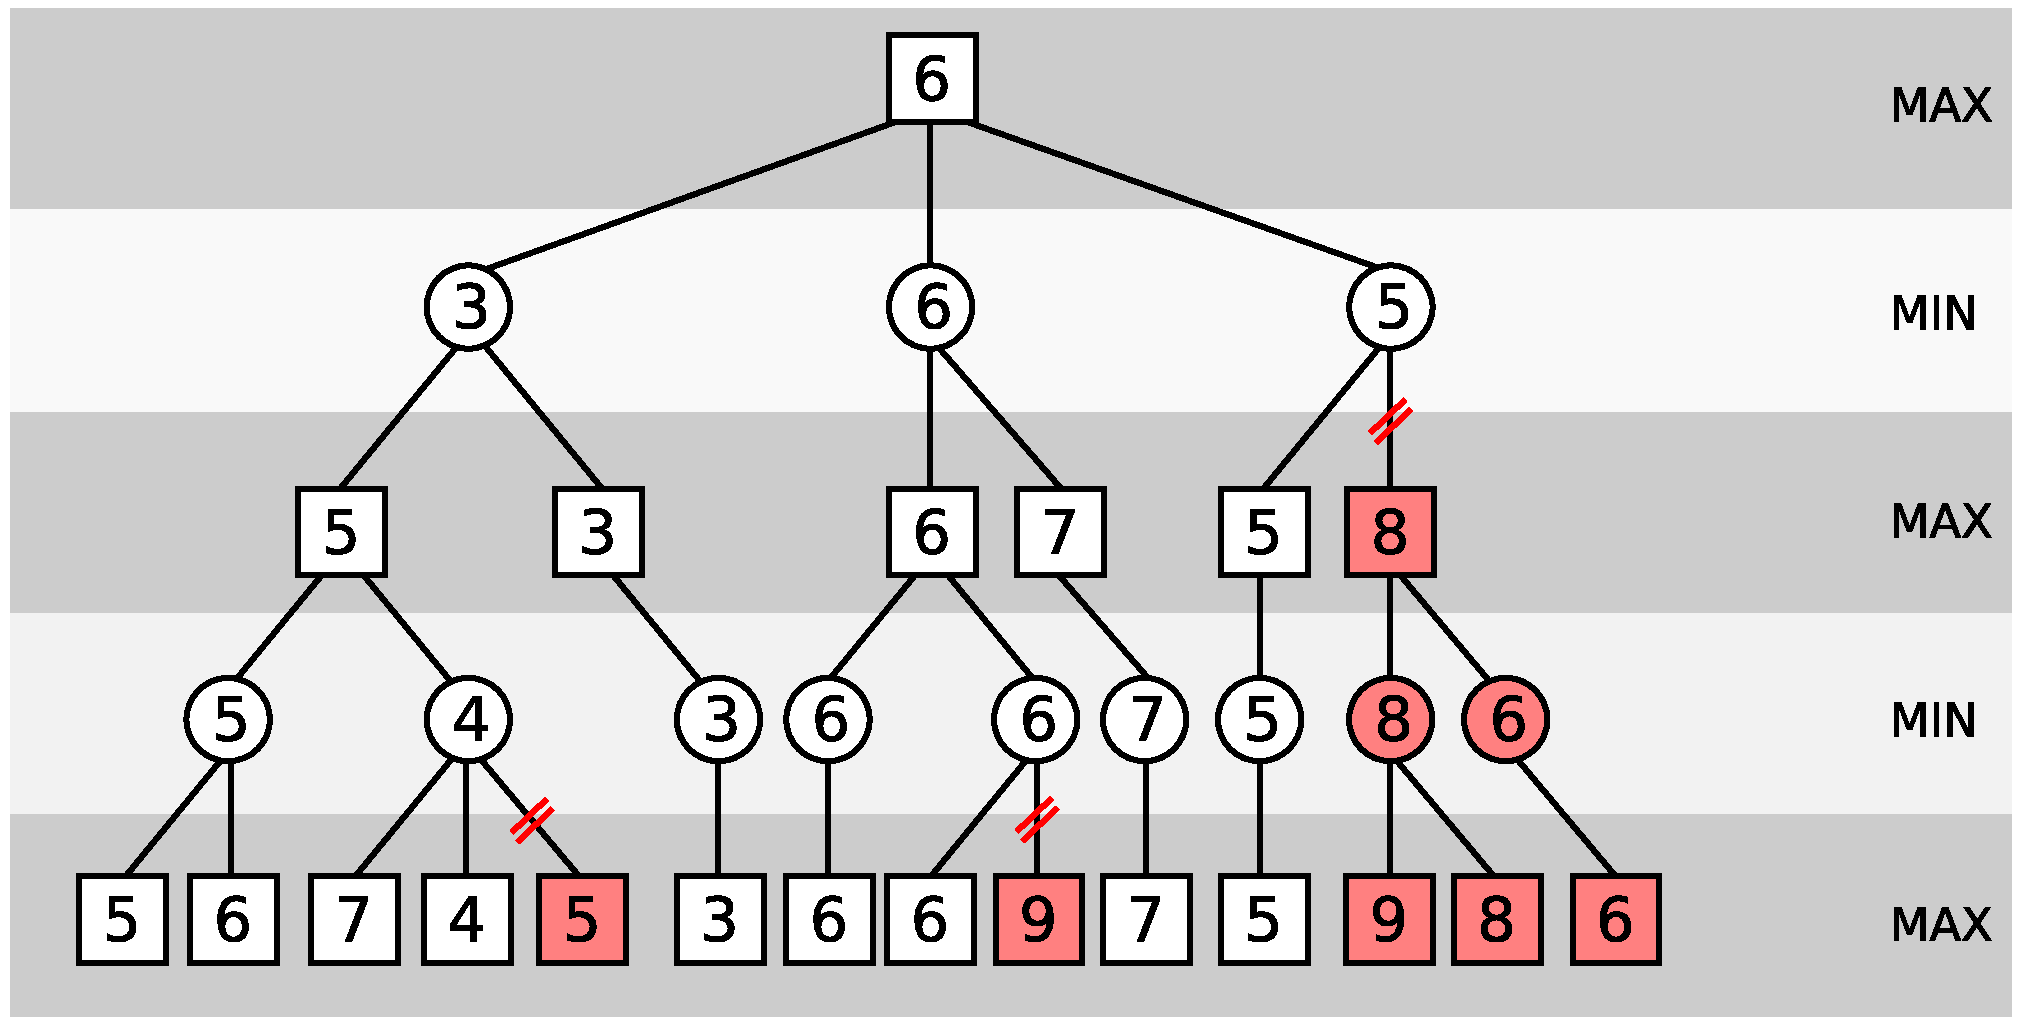
\includegraphics[height=0.6\textheight]{pix/alphabeta}
    \centering
    \caption{
        \st{Minimax}
        \st{Negamax}
        Négamax avec élagage $\alpha\beta$}
  \end{figure}
\end{frame}

\section{Choix d’implémentation}
    \begin{frame}{Modules}
        \begin{columns}
        \begin{column}{.2\textwidth}
            
\includegraphics[width=1\textwidth]{./pix/sym_puzzle}
        \end{column}
        \begin{column}{.8\textwidth}

  \begin{itemize}
    \item \textbf{evaluation.pl} Éval, NégaMax, Alpha/Beta
    \item \textbf{gui.pl} Affichages et interactions.
    \item \textbf{jeu.pl} Prédicats des coups.
    \item \textbf{regles.pl} Règles et conditions de victoire.
    \item \textbf{main.pl} Lance le jeu.
  \end{itemize}
        \end{column}
    \end{columns}
\end{frame}

\begin{frame}{Représentation des données}
\vspace{-.65cm}
    \begin{block}{Coup}
          Liste: \texttt{[Case départ, Case arrivée, Id]}
    \end{block}
    \begin{block}{Plateau}
        Liste de neuf entiers $\in \left\{-1, 0, 1, 2\right\}$, avec:
        \begin{description}
	        \item [-1] : case vide
	        \item [0] : case sans pion
	        \item [1] : pion du joueur 1
	        \item [2] : pion du joueur 2
        \end{description}
        Exemple : \texttt{[1, 1, 2, 0, -1, 0, 1, 0, 0]}
    \end{block}
\end{frame}

\section{Résultats}

\begin{frame}{Utilité de l'élagage Alpha/Beta}
    \begin{columns}
        \begin{column}{.2\textwidth}
            
\includegraphics[width=1.3\textwidth]{./pix/sym_cut}
        \end{column}
        \begin{column}{.6\textwidth}
            \begin{center}
                Sans élagage, une profondeur de 10 fait exploser les calculs.
            \end{center}
        \end{column}
    \end{columns}
\end{frame}

\begin{frame}{Efficacité}
    \begin{columns}
        \begin{column}{.2\textwidth}
            
\includegraphics[width=1.3\textwidth]{./pix/sym_brain}
        \end{column}
        \begin{column}{.6\textwidth}
        \begin{itemize}
            \itemsep2em
	        \item L'IA est imbattable !
	        \item Réponse instantané pour un récursion de 4.
	        \item Quelques secondes pour une récursion de 10.
        \end{itemize}
        \end{column}
    \end{columns}
\end{frame}

\begin{frame}{Questions}
    \begin{columns}
        \begin{column}{.2\textwidth}
            
\includegraphics[width=1.3\textwidth]{./pix/sym_question}
        \end{column}
        \begin{column}{.6\textwidth}
            \begin{center}
                \huge Questions ?
            \end{center}
        \end{column}
    \end{columns}
\end{frame}
\end{document}
